\input{../../preamble2.tex}

\begin{document}
\begin{center}
	\Huge\textbf{Математический анализ}
\end{center}
\tableofcontents
\newpage

 \begin{center}
 \large{\textbf{Модуль №1} \\
 \textit{Элементарные функции и пределы}}
 \end{center}
 \input{Основы математического анализа.tex}
 \newpage
 \zerocounter
 \input{Числовая последовательность.tex}
 \newpage
 \zerocounter
 \input{Предел функции.tex}
 \newpage
 \zerocounter
 \input{бмф. Арифметические операции.tex}
 \newpage
 \zerocounter
 \input{Предел функции. бмф ббф.tex}
 \newpage
 \zerocounter
 \input{Непрерывность функции. Точки разрыва.tex}
 \newpage
 \zerocounter
 \begin{center}
 \large{\textbf{Модуль №2} \\
 \textit{Дифференциальное исчисление функции одной переменной}}
 \end{center}
 \input{Производная функции.tex}
 \newpage
 \zerocounter
 \input{Дифференциал функции.tex}
 \zerocounter
 \newpage
\input{Основные теоремы дифференциального исчисления.tex}
\newpage
\zerocounter
\input{Раскрытие неопределённостей.tex}
\zerocounter
\newpage
%%%%%%%%%%%%%%%%%%%%
\section{Формула Тейлора}
\subsection{Формула Тейлора. Многочлены Тейлора}
\begin{theorem}
	Пусть функция $y=f(x)$ $n$ раз дифференцируема в точке $x_0$ и определена в некоторой окрестности этой точки. Тогда $\forall x \in S(x_0)$ имеет место формула Тейлора:
	\begin{align}
		\begin{aligned}
			f(x) =& f(x_0)  + \frac{f'(x_0)}{1!}\cdot (x-x_0) + \frac{f''(x_0)}{2!}\cdot (x-x_0)^2 + \frac{f'''(x_0)}{3!}\cdot (x-x_0)^3 + \\
			              & + \ldots + \frac{f^{(n)}(x_0)}{n!}\cdot (x-x_0)^n + R_n(x)
		\end{aligned}
	\end{align}
	Кратко: $f(x) = P_n(x) + R_n(x)$, где
	\begin{flalign*}
		&\begin{aligned}
		P_n(x) =& f(x_0)  + \frac{f'(x_0)}{1!}\cdot (x-x_0) + \frac{f''(x_0)}{2!}\cdot (x-x_0)^2 + \frac{f'''(x_0)}{3!}\cdot (x-x_0)^3 + \\
		& + \ldots + \frac{f^{(n)}(x_0)}{n!}\cdot (x-x_0)^n \hspace{2cm} \text{--- многочлен Тейлора}\qquad x\to x_0
		\end{aligned}  &
	\end{flalign*}
	$R_n(x)$ --- остаточный член формулы Тейлора
\end{theorem}
\begin{proof}
	Покажем, что такой многочлен существуеТ.Будем искать многочлен Тейлора в виде:
	\begin{gather}
		P_n(x) = a_0 + a_1(x-x_0) + a_2(x-x_0)^2 + a_3(x-x_0)^3 + a_4(x-x_0)^4 + \ldots + a_n(x-x_0)^n
	\end{gather}
	$a_1, a_2, \ldots, a_n \text{ --- } const$\\ \vspace{-2\topsep}
	\begin{flalign}
		&\text{Пусть выполнено условие: } \left\{\begin{aligned}
			        & P_n(x_0) = f(x_0)                     \\
			        & P'_n(x_0) = f'(x_0)                   \\
			        & P''_n(x_0) = f''(x_0)                 \\
			        & \ldots\ldots\ldots\ldots\ldots\ldots  \\
			        & P^{(n)}_n(x_0) = f^{(n)}(x_0)
		       \end{aligned}\right.&
	\end{flalign}
	$f'(x_0), f''(x_0), \ldots, f^{(n)}(x_0)$ -- существуют, так как $y=f(x)$ $n$ раз дифференцируема в точке $x_0$.\\
	Вычислим $P'_n(x),\ldots,P_n^{(n)}(x)$:
	\begin{flalign*}
		 & P_n(x) = a_0 + a_1(x-x_0) + a_2(x-x_0)^2 + a_3(x-x_0)^3 + a_4(x-x_0)^4 + \ldots + a_n(x-x_0)^n                                                & \\
		 & P'_n(x) = a_1\cdot 1 + a_2\cdot 2(x-x_0) + a_3\cdot 3(x-x_0)^2 + a_4\cdot 4(x-x_0)^3 + \ldots + a_n\cdot n(x-x_0)^{n-1}\hspace*{-7pt}              & \\
		 & P''_n(x) = a_2\cdot 2\cdot 1 + a_3\cdot 3\cdot 2(x-x_0) + a_4\cdot 4\cdot 3(x-x_0)^2 + \ldots + a_n\cdot n\cdot (n-1)(x-x_0)^{n-2}\hspace*{-7pt} & \\
		 & P''_n(x) = a_3\cdot 3\cdot 2\cdot 1 + a_4\cdot 4\cdot 3\cdot 2(x-x_0) + \ldots + a_n\cdot n\cdot (n-1)\cdot (n-2)(x-x_0)^{n-3}              & \\
		 & \ldots \ldots \ldots\ldots\ldots\ldots\ldots\ldots\ldots\ldots\ldots\ldots\ldots\ldots\ldots\ldots\ldots\ldots\ldots\ldots\ldots\ldots\ldots\ldots\ldots\ldots\ldots\ldots                                                                                                                    & \\
		 & P_n^{(n)}(x) = a_n\cdot n(n-1) \cdot (n-2) \cdot\ldots\cdot 1 = a_n \cdot n!
	\end{flalign*} \
	$ x = x_0$
	\begin{flalign*}
		&\left\{\begin{aligned}
			        & P_n(x_0) = a_0                             \\
			        & P'_n(x_0) = 1\cdot a_1                     \\
			        & P''_n(x_0) = 1\cdot 2 \cdot a_2            \\
			        & P'''_n(x_0) = 1\cdot 2 \cdot 3 \cdot a_3   \\
			        & \ldots\ldots\ldots\ldots\ldots\ldots\ldots \\
			        & P^{(n)}_n(x_0) = n!\cdot a_n
		       \end{aligned} \right.\ \overset{(3)}{\Longrightarrow} \left\{
				\begin{aligned}
					& P_n(x_0) = a_0 = f(x_0)                                      \\
					& P'_n(x_0) = 1\cdot a_1 = f'(x_0)                             \\
					& P''_n(x_0) = 1\cdot 2 \cdot a_2 = f''(x_0)                   \\
					& P'''_n(x_0) = 1\cdot 2 \cdot 3 \cdot a_3 = f'''(x_0)         \\
					& \ldots\ldots\ldots\ldots\ldots\ldots\ldots\ldots\ldots\ldots \\
					& P^{(n)}_n(x_0) = n!\cdot a_n = f^{(n)}(x_0)
		        \end{aligned} \right. &
	\end{flalign*}
	\begin{flalign*}
		& \text{Выразим } a_0, a_1, \ldots, a_n\colon \left\{
			\begin{aligned}
		 & a_0 = f(x_0)                  \\
		 & a_1 = \frac{f'(x_0)}{1!}      \\
		 & a_2 = \frac{f''(x_0)}{2!}     \\
		 & a_3 = \frac{f'''(x_0)}{3!}    \\
		 & \ldots\ldots\ldots\ldots      \\
		 & a_n = \frac{f^{(n)}(x_0)}{n!} \\
			\end{aligned}
		\right. &
	\end{flalign*}
	Подставим $a_0, a_1, \ldots, a_n$ в (2):
	\begin{flalign*}
		&\begin{aligned}
		 P_n(x) = f(x_0) &+ \frac{f'(x_0)}{1!}\cdot (x-x_0) + \frac{f''(x_0)}{2!} \cdot(x-x_0)^2 + &\\
		& + \frac{f'''(x_0)}{3!} \cdot (x-x_0)^3 + \ldots + \frac{f^{(n)}(x_0)}{n!} \cdot (x-x_0)^n &
		\end{aligned} \text{ -- многочлен Тейлора}&
	\end{flalign*}
\end{proof}
\begin{theorem}
	Пусть функция $y=f(x)$ $n$ раз дифференцируема в точке $x_0$, тогда
	\begin{gather*}
		x\to x_0\qquad \boxed{R_n (x) = o\big((x-x_0)^n\big)} \text{ --- форма Пеано.}
	\end{gather*}
\end{theorem}
\begin{proof}
	Формула Тейлора: \vspace{-\topsep}
	\begin{flalign*}
		 & f(x) = P_n(x) + R_n(x) & \\
		 & R_n(x) = f(x) - P_n(x) &
	\end{flalign*}
	В силу условия (3):
	\begin{align*}
		 & R_n(x_0) = f(x_0) - P_n(x_0) \xlongequal{\text{(3)}} f(x_0) - f(x_0) = 0 \\
		 & R_n'(x_0) = f'(x_0) - P'_n(x_0) \xlongequal{\text{(3)}} f'(x_0) - f'(x_0) = 0 \\
		 & \ldots \ldots \ldots \ldots\ldots\ldots\ldots\ldots\ldots\ldots\ldots\ldots\ldots\ldots\ldots\ldots\ldots\ldots \\
		 & R_n^{(n)}(x_0) = f^{(n)}(x_0) - P^{(n)}_n(x_0) \xlongequal{\text{(3)}} f^{(n)}(x_0) - f^{(n)}(x_0) = 0
	\end{align*}
	Вычислим:
	\begin{flalign*}
		\lim_{x\to x_0}\frac{R_n(x)}{(x-x_0)^n} &= \left(\frac{0}{0}\right) \xlongequal{\text{Л-Б}} \lim_{x\to x_0}\frac{R_n'(x)}{n\cdot(x-x_0)^{n-1}} = \left(\frac{0}{0}\right) \xlongequal{\text{Л-Б}}\ldots =&\\
		& = \lim\limits_{x \to x_0} \frac{R_n^{(n)}(x)}{n\cdot(n-1)\cdot\ldots\cdot 1}= \frac{1}{n!}\lim\limits_{x \to x_0}R_n^{(n)}(x) = \frac{1}{n!}\cdot R_n^{(n)}(x_0) = \frac{1}{n!} \cdot 0 = 0 &
	\end{flalign*}
	Вывод: $R_n(x) = o\big((x-x_0)^n\big)$ при $x \to x_0$
\end{proof}

\begin{theorem}
	Пусть функция $y=f(x)$ $(n+1)$ раз дифференцируема в $S(x_0)$,\\
	$\forall x \in S(x_0)\colon f^{(n+1)}(x)\ne0$. Тогда: 
	\begin{gather*}
		\underset{\text{форма Лагранжа}}{\boxed{R_n(x) = \frac{f^{(n+1)}(c)}{(n+1)'}\cdot (x- x_0)^{n+1}}, \text{ где } c \in S(x_0)}
	\end{gather*}
\end{theorem}
\begin{proof}
	$f(x) = P_n(x) + R_n(x)$\\
	Будем искать:
	\begin{gather*}
		R_n(x) = \frac{\varphi(x)}{(n+1)!}\cdot(x-x_0)^{n+1}, \text{ где $\varphi(x)$ -- неизвестная функция}
	\end{gather*}
	Вспомогательная функция:
	\begin{flalign*}
		F(t) &= P_n(t) + R_n(t) - f(x) = &\\
		& = f(t) + \frac{f'(t)}{1!}\cdot(x-t) + \frac{f''(t)}{2!}\cdot(x-t)^2 + \ldots + \frac{f^{(n)}(t)}{n!}\cdot(x-t)^n + &\\
		& + \frac{\varphi(x)}{(n+1)!}\cdot(x-t)^{n+1} - f(x),\quad \text{$t$ -- переменная}&
	\end{flalign*} 
	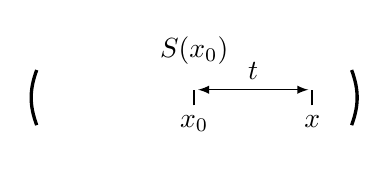
\begin{tikzpicture}[very thick, >=latex]
		\tkzInit[xmin=-2.5, xmax=2.5, ymin=0, ymax=1]
		\tkzDrawX[thick]
		\draw (-2,0.35) to [out=-110, in=110] (-2, -0.35);
		\draw (2,0.35) to [out=-70, in=70] (2, -0.35);
		\draw[thick] (0, -0.1) node[below]{$x_0$}-- (0, 0.1);
		\draw[thick] (1.5, -0.1) node[below]{$x$} -- (1.5, 0.1);
		\draw[thin, <->] (0.05, 0.1) -- (1.45, 0.1) node[midway, above]{$t$};
		\node[above = 8pt] at (0, 0) {$S(x_0)$};
	\end{tikzpicture} \qquad
	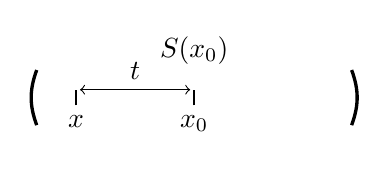
\begin{tikzpicture}[very thick]
		\tkzInit[xmin=-2.5, xmax=2.5, ymin=0, ymax=1]
		\tkzDrawX[thick]
		\draw (-2,0.35) to [out=-110, in=110] (-2, -0.35);
		\draw (2,0.35) to [out=-70, in=70] (2, -0.35);
		\draw[thick] (0, -0.1) node[below]{$x_0$}-- (0, 0.1);
		\draw[thick] (-1.5, -0.1) node[below]{$x$} -- (-1.5, 0.1);
		\draw[thin, <->] (-0.05, 0.1) -- (-1.45, 0.1) node[midway, above]{$t$};
		\node[above = 8pt] at (0, 0) {$S(x_0)$};
	\end{tikzpicture}\\
	Функция $F(t)$ удовлетворяет условию теоремы \textit{Ролля} (\textbf{С.\pageref{Ролль}, Т.\ref{Ролль}}) на $[x_0; x]\ |\ [x; x_0]$
	\begin{enumerate}
		\item $F(t)$ -- непрерывна на $[x_0; x]\ |\ [x; x_0]$.\\
		По условию функция $f(x)$ $(n+1)$ раз дифференцируема в $S(x_0)\ \Rightarrow$ по теореме \textit{о связи дифференцируемости и непрерывности} (\textbf{С.\pageref{Связь диф. и непр. функции}, Т.\ref{Связь диф. и непр. функции}}):\\
		 $f(t), f'(t), \ldots, f^{(n)}(t)$ -- непрерывны на $[x_0; x]\ |\ [x; x_0]$\\
		$F(t)$ -- непрерывна на $[x_0; x]\ |\ [x; x_0]$ как сумма непрерывных функций
		\item $F(t)$ -- дифференцируема на $(x_0; x)\ |\ (x; x_0)$\\
		По условию $y=f(x)$ $(n+1)$ раз дифференцируема в $S(x_0)\ \Rightarrow$\\
		$f(t), f'(t), \ldots, f^{(n)}(t)$ -- дифференцируемы на $(x_0; x)\ |\ (x; x_0)$.\\
		$F(t)$ -- дифференцируема как сумма дифференцируемых функций.
		\item $F(x) = f(x) - f(x) = 0$  
		\begin{flalign*}
			F(x_0) = f(x_0) &+ \frac{f'(x_0)}{1!}\cdot(x-x_0) + \ldots + \frac{f^{(n)}(x_0)}{n!}\cdot(x-x_0)^{n} + &\\
			& + \frac{\varphi(x)}{(n+1)!}\cdot(x - x_0)^{n+1} - f(x) = f(x) - f(x) = 0 &
		\end{flalign*}
		По теореме \textit{Ролля}: $\exists\ c \in (x; x_0)\ |\ c \in (x_0; x)\colon F'(c) = 0$\\
		Вычислим $F'(t)$:
		\begin{flalign*}
			F'(t) = f'(t) &+ \left(\frac{f''(t)}{1!}\cdot(x-t) + \frac{f'(t)}{1!}\cdot(-1)\right) + &\\
			& + \left(\frac{f'''(t)}{2!}\cdot(x-t)^2 + \frac{f''(t)}{2!}\cdot 2 \cdot (x-t) \cdot (-1) \right) + \ldots + &\\
			& + \left(\frac{f^{(n+1)}(t)}{n!}\cdot(x-t)^n + \frac{f^{(n)}(t)}{n!}\cdot n \cdot (x-t)^{n-1}\cdot (-1)\right) + &\\
			& + \frac{\varphi(x)}{(n+1)!}\cdot (n+1) \cdot (x-t)^n \cdot (-1) &
		\end{flalign*}
		\begin{flalign*}
			F'(c) = \frac{f^{(n+1)}(c)}{n!}\cdot (x-c)^n &- \frac{\varphi(x)}{n! \cdot \cancel{(n+1)}}\cdot \cancel{(n+1)} \cdot (x-c)^n = 0 &\\
			\frac{f^{(n+1)}(c)}{n!}\cdot (x-c)^n	&= \frac{\varphi(x)}{n!}\cdot (x-c)^n &\\
			\varphi(x) & = f^{(n+1)}(c),\quad c\in (x_0; x)\ |\ c\in (x; x_0)  &
		\end{flalign*}
		\begin{flalign*}
			& R_n(x) = \frac{f^{(n+1)}(c)}{(n+1)!}\cdot (x-x_0)^{n+1},\quad \forall\ c \in S(x_0) &
		\end{flalign*}
	\end{enumerate}
\end{proof}
Иногда $c = x_0 + \Theta (x-x_0)$\qquad $\Theta$ -- малый параметр \qquad $\Theta \in (0; 1)$
\subsubsection{Формула Тейлора с остаточным членом в форме Пеано}
\begin{gather*}
	f(x) = f(x_0) + \frac{f'(x_0)}{1!}\cdot(x-x_0) + \frac{f''(x_0)}{2!}\cdot(x-x_0)^2 + \ldots + \frac{f^{(n)}(x_0)}{n!}\cdot(x-x_0)^n + o\Big((x-x_0)^{n}\Big)
\end{gather*}
\subsubsection{Формула Тейлора с остаточным членом в форме Лагранжа}
\begin{flalign*}
	f(x) = f(x_0) &+ \frac{f'(x_0)}{1!}\cdot(x-x_0) + \frac{f''(x_0)}{2!}\cdot(x-x_0)^2 + \ldots + \frac{f^{(n)}(x_0)}{n!}\cdot(x-x_0)^n + &\\
	& + \frac{f^{(n+1)}\Big(x_0 + \Theta (x-x_0)\Big)}{(n+1)!}\cdot(x-x_0)^{n+1}
\end{flalign*}
\subsection{Формула Маклорена}
Формула Маклорена --- это частный случай формулы Тейлора при $x_0 = 0$
\begin{gather*}
	f(x) = f(0) + \frac{f'(0)}{1!}\cdot x + \ldots + \frac{f^{(n)}(0)}{n!}\cdot x^n + R_n(x)
\end{gather*}
\begin{flalign*}
	& R_n(x) = o\left(x^n\right)\text{ -- форма Пеано} &\\
	& R_n(x) = \frac{f^{(n+1)}(\Theta x)}{(n+1)!}\cdot x^{n+1} \text{ -- форма Лагранжа} &\\
	& c = x_0 + \Theta(x - x_0)\Big|_{x_0=0} = 0 + \Theta(x - 0) = \Theta x \qquad \Theta \in (0;1)\qquad \Theta \text{ -- малый параметр} &
\end{flalign*}
\subsection{Разложения основных элементарных функций по формулам Маклорена}
\subsubsection{$y=e^x$}
$y = f(x) = e^x,\quad x_0= 0,\quad f(0) = e^0 = 1$
\begin{flalign*}
	& \left\{ \begin{aligned}
		&f'(x) = e^x\\
		&f''(x) = e^x\\
		&f'''(x) = e^x\\
		&\ldots\ldots\ldots\ldots\\
		&f^{(n)}(x) = e^x
	\end{aligned} \right. \longrightarrow\  \left\{ \begin{aligned}
		&f'(0) = 1\\
		&f''(0) = 1\\
		&f'''(0) = 1\\
		&\ldots\ldots\ldots\ldots\\
		&f^{(n)}(0) = 1
	\end{aligned} \right.&\\
	& e^x = 1 + \frac{1}{1!}\cdot x + \frac{1}{2!}\cdot x^2 + \frac{1}{3!}\cdot x^3 + \ldots + \frac{1}{n!}\cdot x^n + R_n(x)\qquad R_n(x) = o\left(x^n\right) \text{ -- форма Пеано} &\\
	& R_n(x) = \frac{f^{(n+1)} (\Theta x)}{(n+1)!}\cdot x^{n+1} = \frac{e^{\Theta x}}{(n+1)!}\cdot x^{n+1} \text{ -- формула Лагранжа}
\end{flalign*}
	\subsubsection*{Следствия:}
	\begin{enumerate}
		\item $\displaystyle{e^{-x} = 1 - \frac{1}{1!}\cdot x + \frac{1}{2!}\cdot x^2	- \frac{1}{3!}\cdot x^3 + \ldots + \frac{(-1)^n}{n!}\cdot x^n + R_n(x) \qquad n=0, 1, 2, \ldots}$
		\item $\displaystyle{ \sh x = \frac{1}{2}\left(e^x - e^{-x}\right) = \frac{1}{1!}\cdot x + \frac{1}{3!}\cdot x^3 + \frac{1}{5!}\cdot x^5 + \ldots + \frac{1}{(2n+1)!}\cdot x^{2n+1} + R_{2n+2}\quad n=0, 1, 2, \ldots}$
		\item $\displaystyle \ch x = \frac{1}{2}\left(e^x+ e^{-x}\right) = 1 + \frac{1}{2!}\cdot x^2 + \frac{1}{4!}\cdot x^4 + \ldots + \frac{1}{(2n)!}\cdot x^{2n} + R_{2n+1} \qquad n=0,1,2, \ldots$
		\item $\displaystyle a^x = 1+\frac{\ln a}{1!}\cdot x + \frac{\ln^2a}{2!}\cdot x^2 + \ldots + \frac{\ln^n a}{n!}\cdot x^n + R_n(x)\qquad n=0, 1, 2,\ldots$
		\item $\displaystyle \sh^2 x = \left(\frac{e^x - e^{-x}}{2}\right)^2 = \frac{1}{4}\cdot \left(e^{2x} - 2 + e^{-2x}\right)  = \frac{1}{2}\cdot \frac{e^{2x} + e^{-2x}}{2} - \frac{1}{2} = \frac{1}{2}\cdot (\ch 2x - 1) $
		\item $\displaystyle \ch^2 x = \left(\frac{e^x + e^{-x}}{2}\right)^2 = \frac{1}{4}\cdot \left(e^{2x}+ 2 + e^{-2x}\right) = \frac{1}{2} \cdot \frac{e^{2x} + e^{-2x}}{2} + \frac{1}{2} = \frac{1}{2}\cdot \left(\ch 2x + 1\right) $
	\end{enumerate}
\subsubsection{$y = \sin x$}
$y = f(x) = \sin x,\ x_0=0$
\begin{flalign*}
	& f(0) = \sin 0 = 0 &\\
	&\left\{ \begin{aligned}
		f'(x) &= \cos x = \sin \left(x + 1\cdot \frac{\pi}{2}\right)\\[1ex]
		f''(x) &= -\sin x = \sin \left(x + 2\cdot \frac{\pi}{2}\right)\\[1ex]
		f'''(x) &= -\cos x = \sin \left(x + 3\cdot \frac{\pi}{2}\right)\\[1ex]
		f^{(IV)}(x) &= \sin x = \sin \left(x + 4\cdot \frac{\pi}{2}\right)\\[1ex]
		f^{(V)}(x) &= \cos x = \sin \left(x + 5\cdot \frac{\pi}{2}\right)\\
		\ldots\ldots&\ldots\ldots\ldots\ldots\ldots\ldots\ldots\ldots\\
		f^{(n)}(x) &= \sin \left(x + n\cdot \frac{\pi}{2}\right) \\
	\end{aligned}\right. \ \longrightarrow\ \left\{\begin{aligned}
		f'(0) &= 1 \\[2.9ex]
		f''(0) &= 0 \\[2.9ex]
		f'''(0) &= -1 \\[2.9ex]
		f^{(IV)}(0) &= 0 \\[2.9ex]
		f^{(V)}(0) &= 1 \\
		\ldots\ldots&\ldots\ldots\ldots \\
		f^{(n)}(0) &= \sin \frac{\pi n}{2} \\
	\end{aligned} \right. &\\[1ex]
	& \sin x = 0 + \frac{1}{1!}\cdot x + \frac{0}{2!}\cdot x^2 - \frac{1}{3!}\cdot x^3 + \frac{0}{4!}\cdot x^4 + \frac{1}{5!}\cdot x^5 + \ldots + \frac{\sin \dfrac{\pi n}{2}}{n!}\cdot x^n + R_n(x)\quad n = 2k,\ k\in \N&\\[1ex]
	& \sin \frac{\pi n}{2} = \left\{ \begin{aligned}
		0,\quad &n = 2k,\ k \in \N \\
		(-1)^{k+1},\quad &n = 2k -1,\ k \in \N
	\end{aligned} \right. &\\[1ex]
	& \sin x = \frac{1}{1!}\cdot x - \frac{1}{3!}\cdot x^3 + \frac{1}{5!}\cdot x^5 + \ldots + \frac{(-1)^{k+1}}{(2k-1)!}\cdot x^{2k-1} + R_{2k}(x) &\\
	& R_{2k}(x) = o\left(x^{2k}\right) &
\end{flalign*}
\begin{flalign*}
	R_{2k}(x) &= R_n(x) = \frac{f^{(n+1)}(\Theta x)}{(n+1)!}\cdot x^{n+1} = \frac{f^{(2k+1)}(\Theta x)}{(2k+1)!} \cdot x^{2k+1} = \frac{\sin \left(\Theta x + (2k+1)\cdot \dfrac{\pi}{2}\right)}{(2k+1)!}\cdot x^{2k+1}= &\\
	& = \frac{\sin \left(\Theta x + \pi k + \dfrac{\pi}{2}\right)}{(2k+1)!}\cdot x^{2k+1} = \frac{\cos \left(\Theta x + \pi k \right)}{(2k+1)!}\cdot x^{2k+1} = \frac{(-1)^k \cdot \cos \Theta x }{(2k+1)!}\cdot x^{2k+1} &\\
\end{flalign*} 
\begin{tikzpicture}[scale=1, very thick]
	\tkzInit[xmin=-2, xmax=2, ymin=-2, ymax=1.5]
	\tkzDrawX[thick] \tkzDrawY[thick]
	\tkzDefPoint(0.8, {sqrt(1.5**2 - 0.8**2)}){plus}
	\tkzDefPoint(-0.8, {-sqrt(1.5**2 - 0.8**2)}){minus}
	\draw (0, 0) circle (1.5);
	\tkzDrawPoint[size = 3pt](plus)
	\tkzDrawPoint[size = 3pt](minus)
	\draw (minus) -- (-0.8, 0) node[midway, right]{\textcircled{$-$}};
	\draw (plus) -- (0.8, 0) node[midway, left]{\textcircled{$+$}};
	\node[above left] at (-1.5, 0) {$\pi$};
	\node[above right] at (1.5, 0) {$2\pi$};
	\node[above] at (-0.8, 0) {$\cos x$};
	\node at (3, 1.5) {$k=1,2,\ldots$};
\end{tikzpicture}
\subsubsection{$y = \cos x$}
$y = f(x) = \cos x,\ x_0=0,\ f(0) = \cos 0 = 1$
\begin{flalign*}
	& f(0) = \cos 0 = 1 &\\
	&\left\{ \begin{aligned}
		f'(x) &= -\sin x= \cos \left(x + 1\cdot \frac{\pi}{2}\right)\\[1ex]
		f''(x) &= -\cos x = \cos \left(x + 2\cdot \frac{\pi}{2}\right)\\[1ex]
		f'''(x) &= \sin x = \cos \left(x + 3\cdot \frac{\pi}{2}\right)\\[1ex]
		f^{(IV)}(x) &= \cos x = \cos \left(x + 4\cdot \frac{\pi}{2}\right)\\[1ex]
		f^{(V)}(x) &= -\sin x = \cos \left(x + 5\cdot \frac{\pi}{2}\right)\\
		\ldots\ldots&\ldots\ldots\ldots\ldots\ldots\ldots\ldots\ldots\\
		f^{(n)}(x) &= \cos \left(x + n\cdot \frac{\pi}{2}\right) \\
	\end{aligned}\right. \ \longrightarrow\ \left\{\begin{aligned}
		f'(0) &= 0 \\[2.9ex]
		f''(0) &= -1 \\[2.9ex]
		f'''(0) &= 0 \\[2.9ex]
		f^{(IV)}(0) &= 1 \\[2.9ex]
		f^{(V)}(0) &= 0 \\
		\ldots\ldots&\ldots\ldots\ldots \\
		f^{(n)}(0) &= \cos \frac{\pi n}{2} \\
	\end{aligned} \right. &\\[1ex]
	& \cos x = 1 + \frac{0}{1!}\cdot x - \frac{1}{2!}\cdot x^2	+ \frac{0}{3!}\cdot x^3 + \frac{1}{4!}\cdot x^4 + \frac{0}{5!}\cdot x^5 + \ldots + \frac{\cos \dfrac{\pi n}{2}}{n!}\cdot x^n + R_n(x)&\\[1ex]
	& \cos \frac{\pi n}{2} = \left\{ \begin{aligned}
		0,\quad &n = 2k-1,\ k \in \N\\
		(-1)^{k},\quad &n = 2k,\ k \in \N
	\end{aligned} \right. &\\[1ex]
	& \cos x = 1 - \frac{1}{2!}\cdot x^2 + \frac{1}{4!}\cdot x^4 + \ldots + \frac{(-1)^k}{(2k)!}\cdot x^{2k} + R_{2k+1}(x)&\\
	& R_{2k+1} (x) = o\left(x^{2k+1}\right)&
\end{flalign*}
\begin{flalign*}
	R_{2k+1}(x) &= R_n(x) = \frac{f^{(n+1)}(\Theta x)}{(n+1)!}\cdot x^{n+1} = \frac{f^{(2k+2)}(\Theta x)}{(2k+2)!}\cdot x^{2k+2} = \frac{\cos \left(\Theta x + (2k+2)\cdot \dfrac{\pi}{2}\right)}{(2k+2)!}\cdot x^{2k+2} = &\\
	& = \frac{\cos (\Theta x + \pi k + \pi)}{(2k+2)!} \cdot x^{2k+2} = \frac{- \cos (\Theta x + \pi k)}{(2k+2)!} \cdot x^{2k+2} = \frac{(-1) \cdot (-1) \cdot \cos \Theta x}{(2k+2)!} \cdot x^{2k+2} = &\\
	& = \frac{(-1)^{k+1}\cdot \cos \Theta x}{(2k+2)!} \cdot x^{2k+2} &
\end{flalign*}
\begin{tikzpicture}[scale=1, very thick]
	\tkzInit[xmin=-2, xmax=2, ymin=-2, ymax=1.5]
	\tkzDrawX[thick] \tkzDrawY[thick]
	\tkzDefPoint(0.8, {sqrt(1.5**2 - 0.8**2)}){plus}
	\tkzDefPoint(-0.8, {-sqrt(1.5**2 - 0.8**2)}){minus}
	\draw (0, 0) circle (1.5);
	\tkzDrawPoint[size = 3pt](plus)
	\tkzDrawPoint[size = 3pt](minus)
	\draw (minus) -- (-0.8, 0) node[midway, right]{\textcircled{$-$}};
	\draw (plus) -- (0.8, 0) node[midway, left]{\textcircled{$+$}};
	\node[above left] at (-1.5, 0) {$\pi$};
	\node[above right] at (1.5, 0) {$2\pi$};
	\node[above] at (-0.8, 0) {$\cos x$};
	\node[below] at (0.8, 0) {$\cos x$};
	\node at (3, 1.5) {$k=1,2,\ldots$};
\end{tikzpicture}

%%%%%%%%%%%%%%%%%%%%
\end{document}